% -------------------------------------------------------------------------------
% Establish page structure & font.
\documentclass[12pt]{report}

\usepackage[total={6.5in, 9in},
	left=1in,
	right=1in,
	top=1in,
	bottom=1in,]{geometry} % Page structure

\usepackage{graphicx} % Required for inserting images
\graphicspath{{../.images/}} % Any additional images I use (BCU logo, etc) are from here.

\usepackage[utf8]{inputenc} % UTF-8 encoding
\usepackage[T1]{fontenc} % T1 font
\usepackage{float}  % Allows for floats to be positioned using [H], which correctly
                    % positions them relative to their location within my LaTeX code.
\usepackage{subcaption}

\usepackage{pdflscape} % Enables the page to be rotated 
                       % landscape for easier image viewing.

% -------------------------------------------------------------------------------
% Declare biblatex with custom Harvard BCU styling for referencing.
\usepackage[
    useprefix=true,
    maxcitenames=3,
    maxbibnames=99,
    style=authoryear,
    dashed=false, 
    natbib=true,
    url=false,
    backend=biber
]{biblatex}

% Additional styling options to ensure Harvard referencing format.
\renewbibmacro*{volume+number+eid}{
    \printfield{volume}
    \setunit*{\addnbspace}
    \printfield{number}
    \setunit{\addcomma\space}
    \printfield{eid}}
\DeclareFieldFormat[article]{number}{\mkbibparens{#1}}

% Declare it as the bibliography source, to be called later via \printbibliography
\addbibresource{litReview.bib}

% -------------------------------------------------------------------------------
% To prevent "Chapter N" display for each chapter
\usepackage[compact]{titlesec}
\usepackage{wasysym}
\usepackage{import}

\titlespacing*{\chapter}{0pt}{-2cm}{0.5cm}
\titleformat{\chapter}[display]
{\normalfont\bfseries}{}{0pt}{\Huge}

% -------------------------------------------------------------------------------
% Custom macro to make an un-numbered footnote.

\newcommand\blfootnote[1]{
    \begingroup
    \renewcommand\thefootnote{}\footnote{#1}
    \addtocounter{footnote}{-1}
    \endgroup
}

% -------------------------------------------------------------------------------
% Fancy headers; used to show my name, BCU logo and current chapter for the page.
\usepackage{fancyhdr}
\usepackage{calc}
\pagestyle{fancy}

\setlength\headheight{37pt} % Set custom header height to fit the image.

\renewcommand{\chaptermark}[1]{%
    \markboth{#1}{}} % Include chapter name.


% Lewis Higgins - ID 22133848           [BCU LOGO]                [CHAPTER NAME]
\lhead{Lewis Higgins - ID 22133848~~~~~~~~~~~~~~~
\includegraphics[width=1.75cm]{BCU}}
\fancyhead[R]{\leftmark}

% ------------------REMOVE ME ----------------------------------------------------

% Temp, using to add notes for the draft edition.
\usepackage{tcolorbox}

% ----------------- REMOVE ME ---------------------------------------------------

\begin{document}

    \makeatletter
    \begin{titlepage}
        
\includegraphics[width=0.3\linewidth]{BCUWide.jpg}\\[4ex]
        \vspace{1cm}
        \begin{center}
            {\huge \bfseries  CMP6200}\\[2ex]
            {\huge \bfseries  Individual Undergraduate Project}\\[2ex]
            {\huge \bfseries 2024 - 2025}\\[6ex]
            {\large \bfseries A2 - Literature Review and Methods}\\[10ex]
            {\huge \bfseries University Artifically Intelligent Assistant}\\[6ex]
            
\includegraphics[width=0.1\linewidth]{Symbol.png}\\[40ex]
            Course: Computer \& Data Science\\
            Student Name: Lewis Higgins\\
            Student Number: 22133848\\
            Supervisor Name: Dr. Atif Azad
        \end{center}
    \end{titlepage}
    \makeatother
    \thispagestyle{empty}
    \newpage

    \tableofcontents
    %\footnotesize{\listoffigures}

    \chapter{Report Introduction}\label{ch:introduction}

    \begin{tcolorbox}[colback=orange!5!white,colframe=orange!75!black,title=Draft notice]
        This is a very early draft of this literature review and will be subject to major change
        over the next month. I've marked sections that I've taken from the proposal, or ones that 
        I'm currently uncertain of, with boxes similar to this one.
    \end{tcolorbox}


    \section{Aims and Objectives}

    \begin{tcolorbox}[colback=red!5!white,colframe=red!75!black,title=Copied from proposal]
        These are still subject to change pending the feedback from my proposal.
    \end{tcolorbox}

    This project aims to aid new and existing students alike while they are attending university with 
    helpful information about the university itself, such as university societies, locations/campuses, 
    and policies through the medium of a digital chatbot companion to converse with.
    Its objectives are to:

    \begin{itemize}
        \item Develop a chatbot capable of accurately answering user queries related to university 
        buildings, policies, and societies with a minimum 95\% accuracy rate.
        \item Conduct a thorough literature review on the surrounding topics, namely AI, LLMs and NLP.
        \item Create effective documentation for all stages of development, highlighting challenges faced during the process.
        \item Manage time effectively to ensure all project milestones are met on a consistent and regular timeframe.
        \item Evaluate the effectiveness of an AI assistant on university student acclimatization.
    \end{itemize}

    \pagebreak % REMOVE ME IF UNNECESSARY

    \section{Literature Search Methodology}

    \begin{tcolorbox}[colback=yellow!5!white,colframe=yellow!75!black,title=Uncertainty]
        I assumed that I should include the exact search terms including special characters
        like asterisks as well as AND + OR queries, but I'm not sure how to best display that
        in this document. I'm also aware that a few of these are parts of each other (Deep learning
        and NLP for example) though I would surely need to research both anyway?
    \end{tcolorbox}

    \noindent All searches performed will be on papers published during or after 2020, due to the 
    constantly evolving fields my project is based on.

    \begin{itemize}
        \item Artifical Intelligence OR AI 
        \begin{itemize}
            \item AND Ethics
            \begin{itemize}
                \item AND Bias
                \item AND Fairness
                \item AND Privacy
            \end{itemize}
        \end{itemize}
        \item Chatbot OR Digital assistant
        \item Large Language Model* OR LLM
        \begin{itemize}
            \item AND fine tuning
        \end{itemize}
        \item Natural Language Processing OR NLP
        \begin{itemize}
            \item Intent recognition
            \item Entity extraction
        \end{itemize}
        \item Deep learning
        \item User Experience OR UX
        \begin{itemize}
            \item AND Design
        \end{itemize}
        \item Information retrieval
    \end{itemize}


    \chapter{Literature Review}

    \section{Themes}

    \section{Review of Literature}

    \subsection{Review}

    Check the template document because I'm not too sure if it's formatted this way.

    \subsection{Theory}

    Check the template document because I'm not too sure if it's formatted this way.
    
    \section{Summary}

    
    \begin{landscape}

    \chapter{Appendix}
    
    \begin{tcolorbox}[colback=red!5!white,colframe=red!75!black,title=Copied from proposal]
        This is still subject to change pending the feedback from my proposal.
    \end{tcolorbox}

    \section{Gantt Chart}



    \begin{figure}[H]
        \centering
        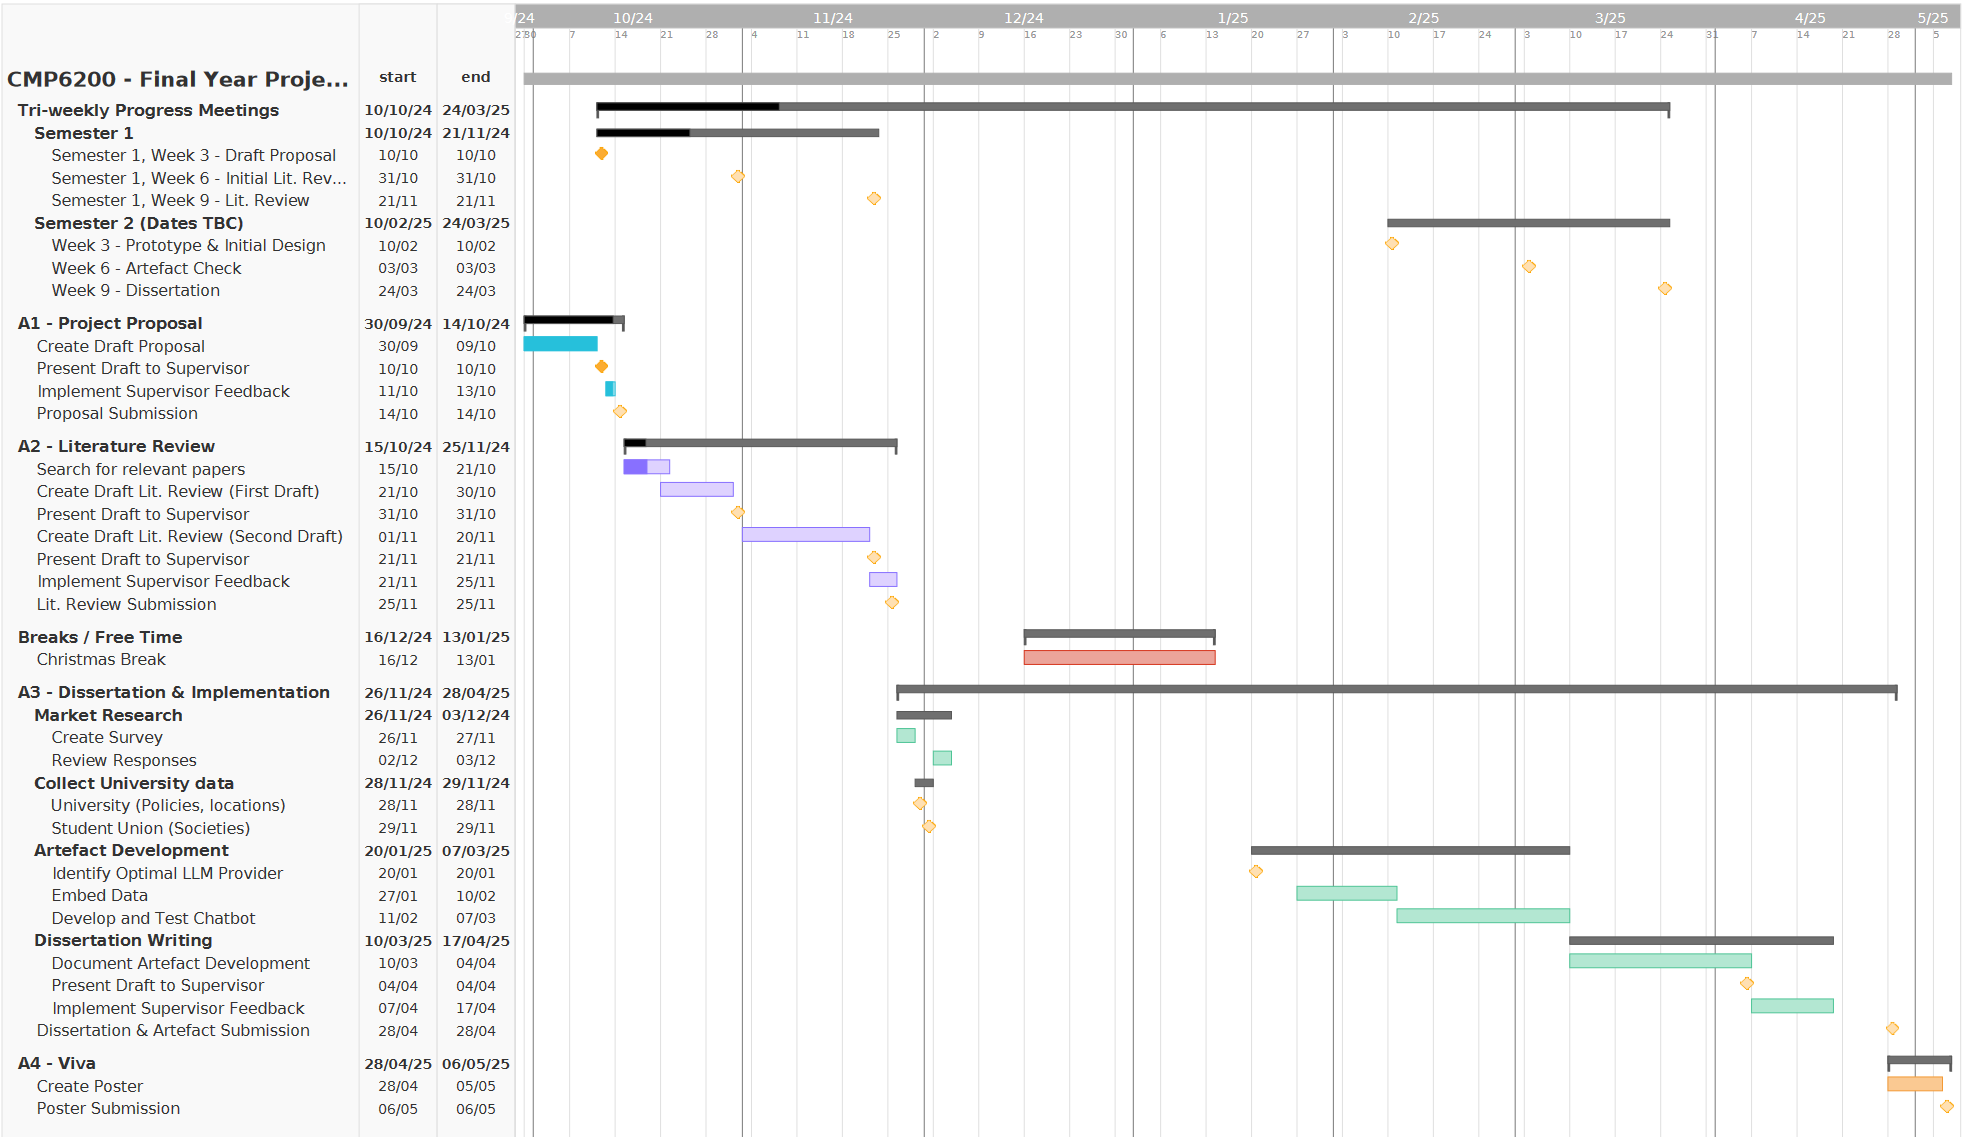
\includegraphics[width=.75\linewidth]{ProposalGantt.png}
        \caption{A conceptual Gantt chart of a development timeline.}
        \label{fig:gantt}
    \end{figure}

    \end{landscape}

    \chapter{References}

    References and bibliographies aren't the same thing. Your references 
    are your directly cited sources, whereas your bibliography is everything you 
    consulted for information, even if you didn't directly cite it. \\

    \noindent \url{https://en.wikibooks.org/wiki/LaTeX/Bibliographies_with_biblatex_and_biber#Splitting_into_different_topics}
    \\ \noindent \large \textbf{That link shows how you can add a "keyword"
    entry to the bibliography entries. In doing so, you could add a "refs" keyword for your 
    references, and a "bib" for your bibliography.}

    \printbibliography

\end{document}